\section{Instrumental Noise}
Currently, the main problem in extracting the GW background is the high instrumental noise.
\subsection{LIGO, Virgo \& KAGRA}

\begin{figure}[h]
    \centering
    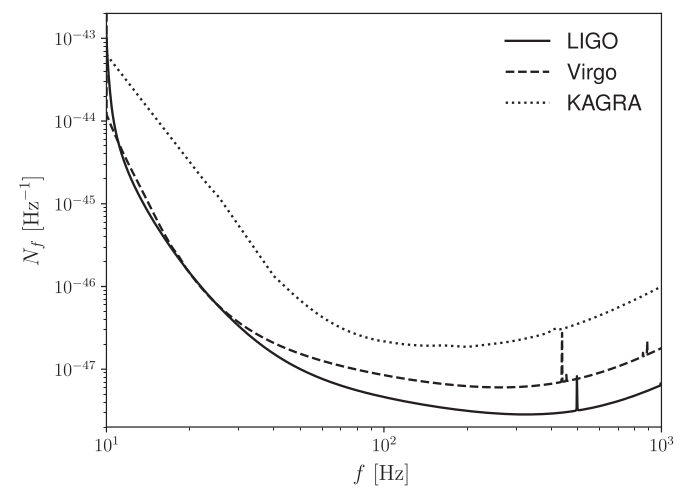
\includegraphics[width=0.7\linewidth]{Images/lvk_frequency_noise.png}
    \caption{Design sensitivity curves for the LVK detector network. For LIGO, this is the advanced LIGO A+ design sensitivity and for Virgo the O5 sensitivity.}
    \label{lvk_sensitivity}
\end{figure} 

\begin{figure}[h]
    \centering
    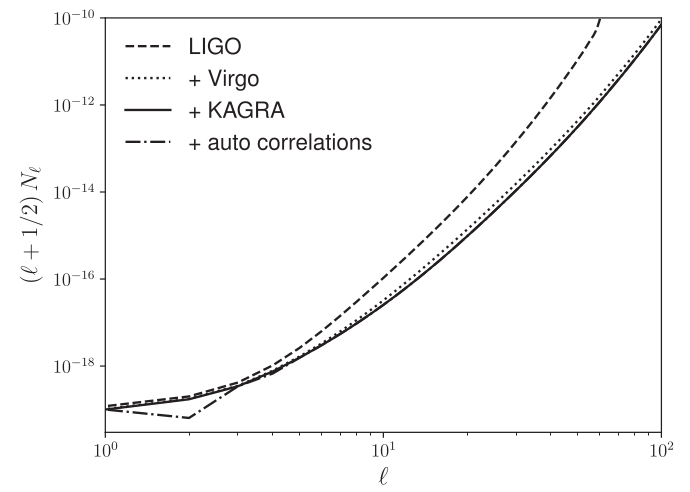
\includegraphics[width=0.7\linewidth]{Images/alonso_ligo_noise.png}
    \caption{The noise angular power spectrum for LVK.}
    \label{lvk_Cl}
\end{figure} 

As can be seen in Fig.\ref{lvk_Cl}, using cross-correlations between the ground-based detectors improves the sensitivity, especially at higher multipoles. Adding auto-correlations of the detectors mostly influences $\ell=2$, which is due to the L-shaped geometry of the detectors. 

\subsection{Einstein Telescope \& Cosmic Explorer}
\begin{figure}[h]
    \centering
    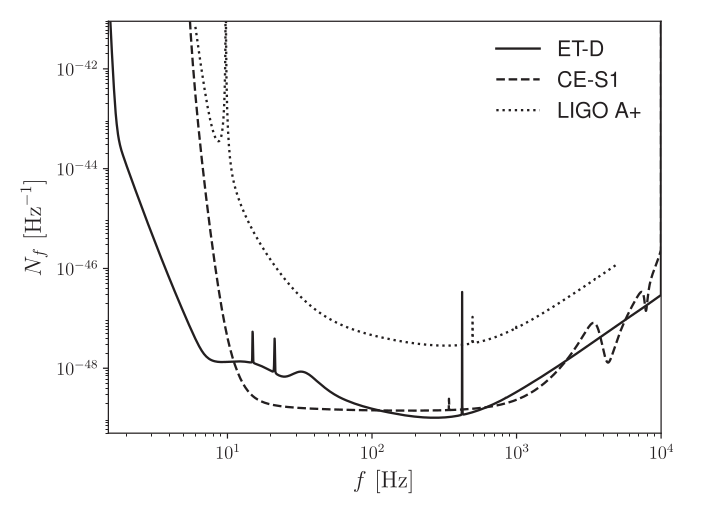
\includegraphics[width=0.7\linewidth]{Images/ET_CE_frequency_noise.png}
    \caption{The design sensitivity curve for ET and CE compared to LIGO A+.}
    \label{ET_sensitivity}
\end{figure} 

The planned ground-based detectors Einstein Telescope (ET) and Cosmic Explorer (CE) will improve the sensitivity by 1-2 orders of magnitude, see Fig.\ref{ET_sensitivity}.

\begin{figure}[h]
    \centering
    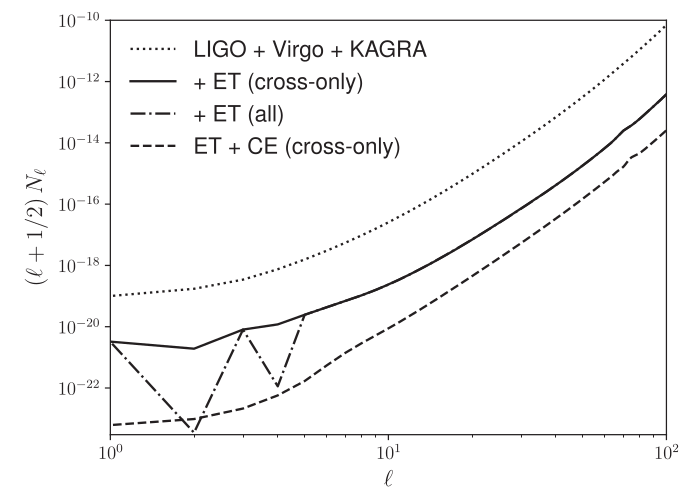
\includegraphics[width=0.7\linewidth]{Images/et_ce_Cl_noise.png}
    \caption{SFR for star-forming galaxies for different redshifts. The velocity at the historical peak halo mass corresponds to the standard halo mass, see equation \ref{v_mpeak-M_h-relation}.}
    \label{ET_Cl}
\end{figure} 

Using the cross-correlations between ET and CE, see Fig.\ref{ET_Cl}, the noise angular power spectrum is expected to drop from $10^{-19}$ to $\approx 6\cdot 10^{-24}$ for the dipole $\ell =1$. Here again, the improvement coming from the auto-correlation is due to the detector shape.


\subsection{LISA \& TianQin}

\begin{figure}[h]
    \centering
    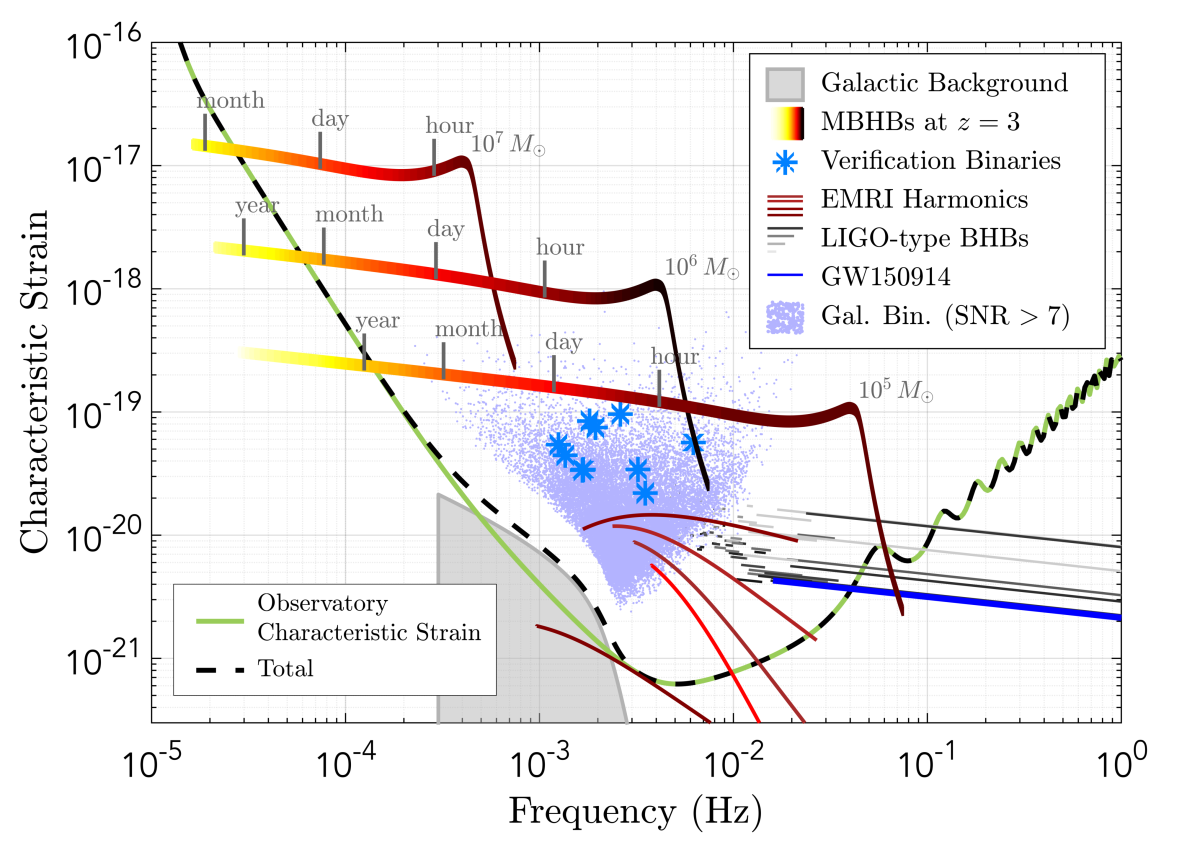
\includegraphics[width=0.7\linewidth]{Images/lisa_frequency_sensitivity.png}
    \caption{Expected sensitivity for LISA. The figure is taken from the LISA L3 mission proposal.}
    \label{LISA_F_sensitivity}
\end{figure} 

\section{Internal Linear Combination?}
\textit{Lorenzo's paper, why we can't use it}